%
% Exemplo LaTeX de artigo UNISINOS
%
% Elaborado com base nas orientações dadas no documento
% ``GUIA PARA ELABORAÇÃO DE TRABALHOS ACADÊMICOS''
% disponível no site da biblioteca da Unisinos.
% http://www.unisinos.br/biblioteca
%
% Os elementos textuais abaixo são apresentados na ordem em que devem
% aparecer no documento.  Repare que nem todos são obrigatórios - isso
% é devidamente indicado em cada caso.
%
% Comentários abaixo colocados entre aspas (`` '') foram
% extraídos diretamente do documento da biblioteca.
%
% Este documento é de domínio público.
%

%=======================================================================
% Declarações iniciais identificando a classe de documento e
% selecionando alguns pacotes adicionais.
%
% As opções disponíveis (separe-as com vírgulas, sem espaço) são:
% - twoside: Formata o documento para impressão frente-e-verso
%   (o default é somente-frente)
% - english,brazilian,french,german,etc.: idiomas usados no documento.
%   Deve ser colocado por último o idioma principal.
%=======================================================================
\documentclass[twoside,english,brazilian]{UNISINOSartigo}
\usepackage[utf8]{inputenc} % charset do texto (utf8, latin1, etc.)
\usepackage[T1]{fontenc} % encoding da fonte (afeta a sep. de sílabas)
\usepackage{graphicx} % comandos para gráficos e inclusão de figuras
\usepackage{bibentry} % para inserir refs. bib. no meio do texto
\usepackage{url} % para mostrar url dos sites referenciados

%=======================================================================
% Escolha do sistema para geração de referências bibliográficas.
%
% O default é usar o estilo unisinos.bst.  Comente a definição abaixo
% e descomente a linha seguinte para usar o estilo do ABNTeX (é
% necessário ter esse pacote instalado).
%
% A vantagem do unisinos.bst é que ele permite o uso de um arquivo .bib
% seguindo as orientações tradicionais do BibTeX (veja essas orientações
% em http://ctan.tug.org/tex-archive/biblio/bibtex/contrib/doc/btxdoc.pdf).
% Entretanto, o estilo não suporta algumas citações mais exóticas como
% apud.  Para isso, use o ABNTeX, mas esteja ciente de que muitas de
% suas referências serão incompatíveis com os estilos tradicionais do
% BibTeX como plain, alpha, ieeetr, entre outros.
%=======================================================================
\unisinosbst
%\usepackage[alf]{abntcite}

%=======================================================================
% Informações Pessoais
%=======================================================================
\title{Proposta de gamificação nos testes de software}

\author{Cássio Linden Albert}
\authorinfo{Aluno do curso de Sistemas de Informação. Email: cassiola@edu.unisinos.br}
\degree{Bacharel em Sistemas de Informação}
\course{Curso de Sistemas de Informação}
\address{São Leopoldo}
\date{2019}

\advisor{Cristiano Bonato Both}
% [Prof. Dr.]
\advisorinfo{Professor da Unisinos. Email: cboth@unisinos.br}

%=======================================================================
% Início do documento.
%=======================================================================
\begin{document}

\maketitle

%=======================================================================
% Resumo em Português.
%
% A recomendação é para 150 a 250 palavras.
%=======================================================================
\begin{abstract}

Hoje, o nível de exigência em aplicações por parte dos usuários está cada vez maior, e os testes de software têm um papel fundamental neste processo. Várias técnicas são usadas pelos profissionais, mas a maioria delas são repetitivas, como, por exemplo, a análise de valor limite. Para mudar esse panorama, propõe-se o uso da gamificação, que traz elementos de jogos em contextos organizacionais, como entregas de projetos, por exemplo. As pesquisas nessa área são relativamente recentes, e está em constante crescimento, conforme indicado em pesquisas na base de dados do Scopus. Os resultados obtidos pelos pesquisadores são animadores, visto que há um indicativo de que a produtividade do profissional aumenta com o uso da gamificação, porém, sua implantação em grandes empresas pode ser difícil.
\palavraschave{gamificação, testes, engenharia de software}
\end{abstract}

%=======================================================================
% Introdução
%=======================================================================
\section{Introdução}

Com a facilitação do acesso à tecnologia, cada vez mais pessoas têm acesso a, ao menos, um smartphone. Consequentemente, mais aplicações estão sendo desenvolvidas e utilizadas com mais frequência. Com isso, a exigência de qualidade dos usuários também cresceu. Vendo esse cenário, os desenvolvedores de software estão colocando a qualidade de seu produto como umas de suas maiores prioridades, e o teste de software tem um papel fundamental neste processo.

Como é sabido, nenhum software está livre de problemas, e muitos detalhes que passam despercebidos pelos desenvolvedores, não passam no crivo de um bom testador. Para isso acontecer, técnicas dos mais variados tipos precisam ser postas em prática para o mínimo de problemas possível chegar ao usuário. Essas técnicas, em boa parte, são bastante repetitivas, o que pode acabar no desgaste e até tédio no profissional de testes. Para resolver isso, várias pesquisas relacionadas à aplicação da gamificação na área de testes têm sido feitas. A gamificação consiste em inserir elementos de jogos em contextos onde os mesmos não estão presentes. Para muitos pesquisadores, essa parece ser a solução para o tédio no trabalho, e um grande incentivador na produtividade do profissional.

Neste artigo será proposto uma forma de atrair testadores manuais para a área de testes automatizados de forma intuitiva, mesmo que este profissional tenha pouca experiência com desenvolvimento de software, com o auxílio de elementos de gamificação.
 

%=======================================================================
% Escrevendo o Texto
%=======================================================================

\section{Fundamentação Teórica}

Esta seção visa abordar alguns dos termos que serão importantes no entendimento da análise feita neste trabalho. Começa abordando a definição de gamificação, segue em suas subseções abordando a definição de teste de software, técnicas e níveis de teste, encerrando com uma breve definição sobre \textit{framework}.

\subsection{Gamificação}

Gamificação é uma forma de inserir elementos de jogos num processo totalmente fora desse contexto \cite{Dale}. Ela está sendo usada para incentivar, motivar e melhorar a desempenho de uma empresa, ou para ajudar no ensino de algum tópico, por exemplo, deixando a atividade mais atrativa para as pessoas. Para \cite{DeJesus}, ``gamificação é um meio promissor para a resolução de problemas de teste'' e ``pode trazer prazer para o desenvolvimento de software.'' Para \cite{Elgrably}, uma das grandes vantagens do uso da gamificação na educação é ``fornecer um sistema no qual os estudantes podem visualizar os efeitos de suas ações e aprendendo conforme a atividade acontece, deixando mais fácil o entendimento da relação das partes com o todo.'' 


\subsubsection{Elementos e mecânicas}

Alguns elementos a ser implementados são essenciais para considerar um processo gamificado. Entre os mais comuns estão: pontos, conquistas, níveis, missões, jornadas (um conjunto de missões), quadro de líderes, notificações (para motivar o jogador diante de uma ação correta) e mecânicas anti-jogo (para limitar até onde um comportamento pode ser recompensado) \cite{Dale}.

Além desses elementos, deve ser considerada a motivação de cada pessoa, e ela pode ocorrer das seguintes maneiras:

\begin{itemize}
	\item a expressão, onde as pessoas são motivadas e recompensadas por mostrar quem elas são (redes sociais são grandes exemplos disso);
	\item a competição, onde as pessoas disputam entre si (ou com elas mesmas);
	\item a exploração, onde as pessoas são motivadas por ter cada vez mais informações sobre algum conteúdo;
	\item e a colaboração, onde as pessoas são motivadas por se sentir parte do todo, através de projetos colaborativos;
\end{itemize}

Também é importante ressaltar que recompensas intrínsecas (como o aprendizado e contribuição para o todo), geralmente, contribuem mais para motivação de uma pessoa do que uma recompensa extrínseca (como dinheiro e selos, por exemplo). A próxima subseção irá tratar sobre testes de software, que é uma parte do fluxo de desenvolvimento de software que pode se beneficiar bastante da gamificação.


\subsection{Teste de software}

Há várias definições possíveis para teste de software, sendo que mais comumente pode ser citado como ``um processo de executar um software com a intenção de encontrar defeitos'' \cite{Myers-1979}, ou verificar se o software está fazendo o que deveria de acordo com seus requisitos \cite{RiosMoreira-2002}. Para o ISTQB (\textit{International Software Testing Qualification Board}), é ``o processo que consiste em todas as atividades do ciclo de vida, tanto estáticas quanto dinâmicas, preocupado com a preparação, planejamento e avaliação de produtos de software e produtos de trabalho relacionados para determinar que eles atendem os requisitos especificados, para demonstrar que eles cumprem sua finalidade e para detectar defeitos.'' \cite{ISTQB-Glos12}

\subsubsection{Técnicas de teste}
Entre as técnicas de teste é possível citar as funcionais e as estruturais. As técnicas funcionais, também conhecidas como teste da caixa-preta, são baseadas num software que já está implementado, em que o usuário (ou um testador) testa se as funcionalidades do programa condizem com os requisitos. Entre as empresas que têm uma estrutura de testes, esta é a técnica mais comum de ser utilizada, apesar de não ser a mais eficiente na resolução de certos tipos de bugs, por exemplo. 

As técnicas estruturais, conhecidas como ``caixa-branca'', são baseadas no código do software desenvolvido. Diferente das técnicas funcionais, esses testes são comumente feitos pelos programadores, e não testam as funcionalidades propriamente ditas. O mais comum de ocorrer é a verificação de comunicação entre os componentes, se o código segue boas práticas, se está bem otimizado, etc.  

As técnicas baseadas em falhas, mais conhecidas como teste de mutação, consistem no desenvolvedor inserir erros no software propositalmente para verificar como ele irá se comportar, além de ser bastante utilizado pelos profissionais de teste para aprimorar casos de teste automatizados. Para esses casos, têm-se os mutantes, que são os programas modificados, e têm os casos de testes já desenvolvidos. Se esses casos de testes consigam detectar os mutantes, diz-se que este caso ``matou'' o mutante. Porém, nessa técnica, deve-se ter cuidado com os mutantes equivalentes, que são alterações em que o resultado da execução será o mesmo, com ou sem o equivalente, pois eles precisariam ser analisados a fim de verificar, de forma manual, se eles são ou não equivalentes \cite{guilhon_2015}. Isso elimina a praticidade de uma das formas mais práticas de detectar mutantes, que é através de testes automatizados. 


\subsubsection{Níveis de teste}
Há três principais níveis de teste: de unidade, de integração e de sistema. Os testes de unidade fazem parte dos testes de caixa-branca, onde trechos específicos do código são testados, como métodos. Como esse tipo de teste se faz no código-fonte, ele deve ser feito pelo desenvolvedor. Tem como regra ser automatizado e reproduzível.

Os testes de integração também fazem parte dos testes de caixa-branca, onde se verifica se a comunicação entre todos componentes do software implementado está funcionando corretamente, ou até mesmo a integração entre softwares diferentes. É feito após os testes de unidade e, diferente dele, os testes de integração pode envolver a equipe de testes. Os testes de sistema testam toda a aplicação desenvolvida, simulando um usuário final em todos os aspectos: desde a forma de uso até o ambiente, que deve ser o mais próximo possível que o usuário final terá. A próxima subseção abordará de forma breve os \textit{frameworks}.


\subsubsection{\textit{Framework}}

Entende-se um \textit{Framework} como uma solução única para problemas que são semelhantes, sendo implementada de forma diferente em cada problema, visto que ele deve ser flexível e extensível para isso. No contexto de desenvolvimento de software, o \textit{framework} é uma aplicação quase completa, cujos os ``pedaços'' faltantes serão implementados pelo desenvolvedor que utilizará o \textit{framework} como base para sua aplicação \cite{ufcg}. A próxima seção irá abordar os trabalhos relacionados com a proposta deste artigo e como se chegou neles.


\section{Trabalhos relacionados}

\subsection{Metodologia de pesquisa}

Para come\c{c}ar esse trabalho, foi feita uma pesquisa sistem\'{a}tica, cujo objetivo foi confirmar que a gamifica\c{c}\~{a}o nos testes de software \'{e} um tema relevante. Para isso, utilizou-se a ferramenta Scopus, que \'{e} um grande reposit\'{o}rio de cita\c{c}\~{o}es e resumos revisados por especialistas das mais diversas \'{a}reas, oferecendo  v\'{a}rias estat\'{i}sticas e gr\'{a}ficos. Para os artigos utilizados nesse trabalho, os seguintes termos foram pesquisados:

\textit{( TITLE-ABS-KEY ( gamification ) AND TITLE-ABS-KEY ( software AND testing ) )AND ( LIMIT-TO ( PUBYEAR , 2019 ) OR LIMIT-TO ( PUBYEAR , 2018 ) OR LIMIT-TO( PUBYEAR , 2017 ) OR LIMIT-TO ( PUBYEAR , 2016 ) OR LIMIT-TO ( PUBYEAR ,2015 ) ) AND ( LIMIT-TO ( SUBJAREA , ``COMP'' ) )}

Essa \textit{query} de pesquisa filtra artigos publicados entre 2015 e 2019 que envolvem termos estritamente relacionados a gamifica\c{c}\~{a}o e testes de software, limitando-se \`{a} \'{a}rea da computa\c{c}\~{a}o. Em 9 de abril de 2019, a \textit{query} retornou 49 resultados. A figura 1 traz um gr\'{a}fico mostrando o n\'{u}mero de artigos publicados desde 2015. Considerando que a pesquisa foi feita no in\'{i}cio de 2019, essa curva tem uma leve queda, mas a tend\^{e}ncia de crescimento nesta \'{a}rea \'{e} grande.

%\pagebreak
%\clearpage
%\newpage

\begin{figure}[!htbp]
	\caption{Curva de artigos publicados de 2015 a 2019}
	\label{fig:imagens/pubByYear.png}
	\centering%
	%\begin{minipage}{.6\textwidth}
		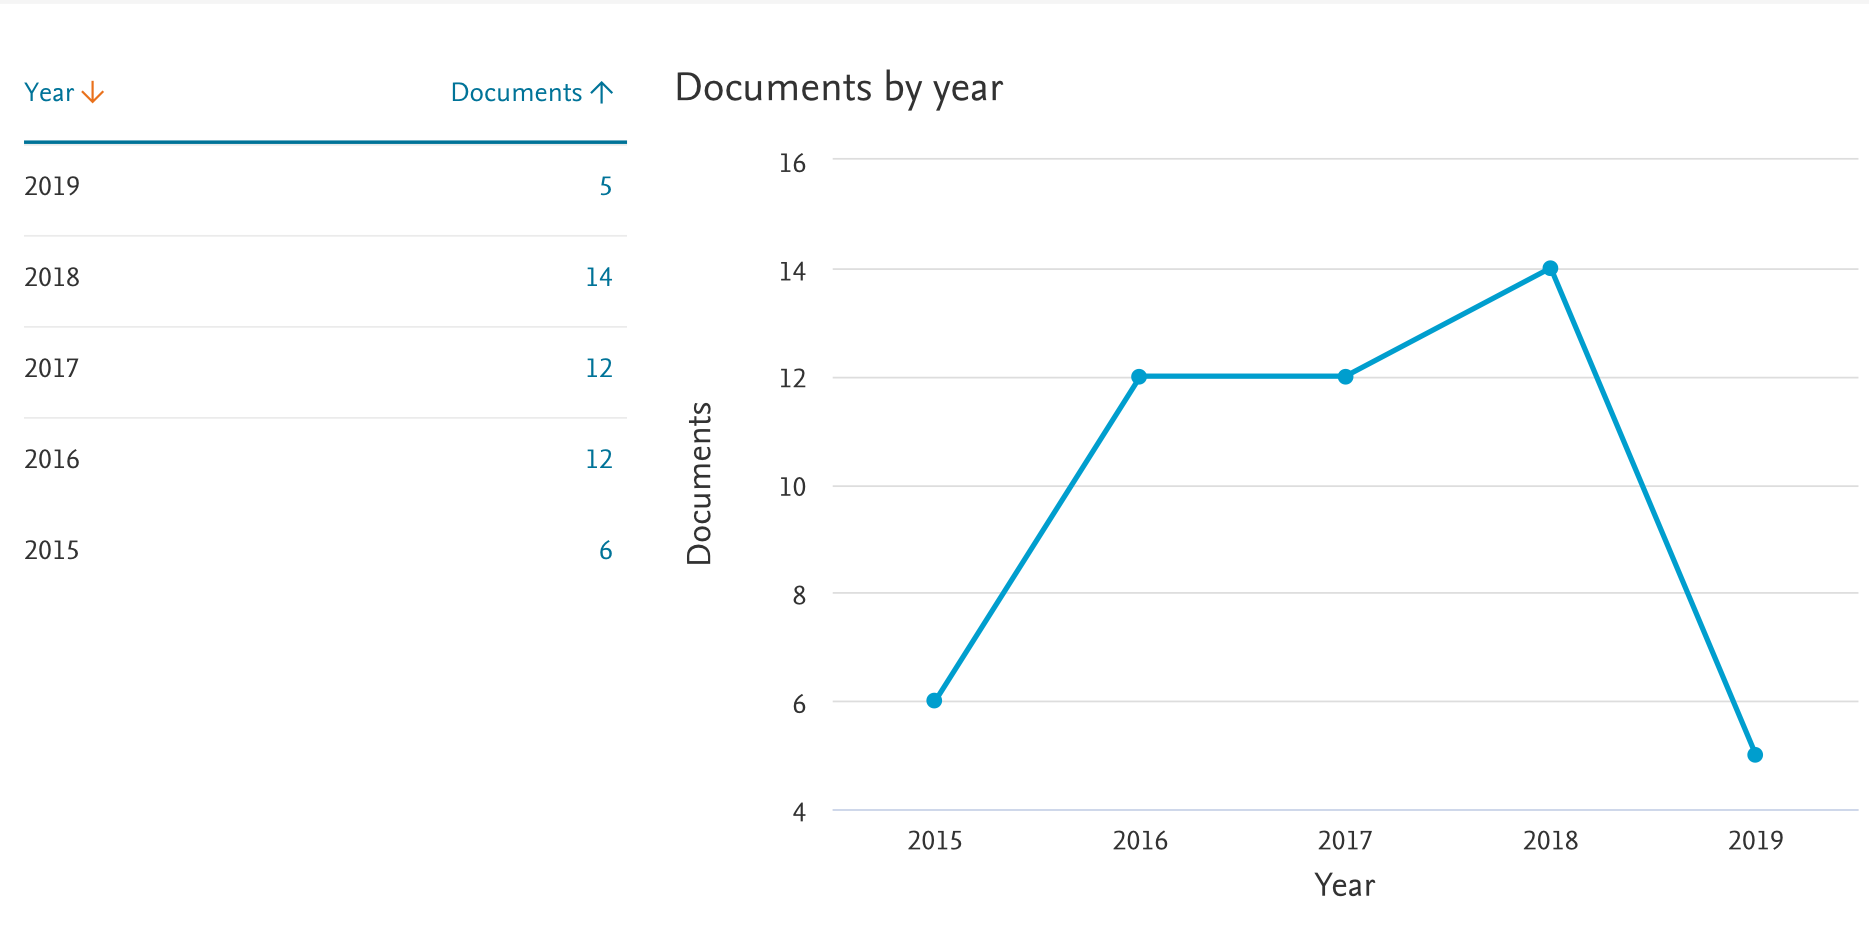
\includegraphics[width=\textwidth]{imagens/pubByYear.png}
	%\end{minipage}
	\begin{center}
        Fonte: Scopus
    \end{center}
\end{figure}

Para selecionar os artigos que ser\~{a}o abordados nessa pesquisa, foram verificados os t\'{i}tulos de cada artigo retornado pela \textit{query} pesquisada no Scopus que tivesse rela\c{c}\~{a}o direta com o t\'{o}pico desejado, passando pela leitura do resumo de cada um e a verifica\c{c}\~{a}o da disponibilidade dos mesmos na base de dados da UNISINOS. Após a leitura dos artigos, os mesmos foram divididos em três categorias: Estudo, \textit{Framework} e Jogo. Esta an\'{a}lise resultou na tabela 1:

%\pagebreak
%\clearpage
\newpage

\begin{table}[]
\caption{Artigos selecionados}
\begin{tabular}{|l|l|l|l|}
\hline
\textbf{Autores} & \textbf{Título} & \textbf{Ano} & \textbf{Categoria} \\ \hline
Fraser G. & Gamification of software testing & 2017 & Estudo \\ \hline
\begin{tabular}[c]{@{}l@{}}De Jesus G.M., Ferrari F.C.,\\ De Paula Porto D.,\\ Fabbri S.C.P.F.\end{tabular} & \begin{tabular}[c]{@{}l@{}}Gamification in software testing:\\ A characterization study\end{tabular} & 2018 & Estudo \\ \hline
\begin{tabular}[c]{@{}l@{}}Elgrably I.S.,\\ Oliveira S.R.B.\end{tabular} & \begin{tabular}[c]{@{}l@{}}Gamification and evaluation of\\ the use the agile tests in software\\ quality subjects: The application\\ of case studies\end{tabular} & 2018 & Estudo \\ \hline
\begin{tabular}[c]{@{}l@{}}Pedreira O., García F.,\\ Brisaboa N., Piattini M.\end{tabular} & \begin{tabular}[c]{@{}l@{}}Gamification in software\\ engineering - A systematic mapping\end{tabular} & 2015 & Estudo \\ \hline
Parizi R.M. & \begin{tabular}[c]{@{}l@{}}On the gamification of\\ human-centric traceability tasks in\\ software testing and coding\end{tabular} & 2016 & Framework \\ \hline
\begin{tabular}[c]{@{}l@{}}García F., Pedreira O.,\\ Piattini M., Cerdeira-\\ Pena A., Penabad M.\end{tabular} & \begin{tabular}[c]{@{}l@{}}A framework for gamification\\ in software engineering\end{tabular} & 2017 & Framework \\ \hline
Houshmand M., Paydar S. & \begin{tabular}[c]{@{}l@{}}EMVille: A gamification-based\\ approach to address the\\ equivalent mutant problem\end{tabular} & 2017 & Framework \\ \hline
Rojas J.M., Fraser G. & \begin{tabular}[c]{@{}l@{}}Code Defenders: A Mutation\\ Testing Game\end{tabular} & 2016 & Jogo \\ \hline
\end{tabular}
\begin{center}
    Fonte: elaborada pelo autor
\end{center}
\end{table}

Na subseção ``discussão dos trabalhos'', os artigos filtrados ser\~{a}o brevemente abordados, considerando suas respectivas categorias.

\subsection{Discussão dos trabalhos}
\subsubsection{Estudo}

\cite{Fraser01} elenca alguns problemas no âmbito do desenvolvimento de software que testes feitos de forma inadequada podem causar, e explora uma forma de melhorar o trabalho do testador: a gamificação. Ele afirma que o uso dessa técnica pode ajudar no trabalho em equipe e no ensino de testes de software nas escolas, além de melhorar a qualidade dos testes.

\cite{DeJesus} apresentaram um cenário geral de outros artigos que abordam gamificação nos testes de software. Esses artigos foram aplicados na indústria e na educação; os elementos abordados foram pontos, emblemas e quadro de líderes; os objetivos eram o desenvolvimento da criatividade, colaboração, engajamento, motivação e satisfação; as técnicas de teste citadas foram a funcional, estrutural e baseados em falhas, sendo a última a mais utilizada; os níveis de teste elencados foram os de unidade, integração e de sistema. Apesar de estarem focado nos testes, os autores afirmam que praticamente todos os artigos estudados por eles podem ser aplicados em todo o processo, com exceção do planejamento e na configuração de dados e ambiente.

\cite{Elgrably} trouxeram um estudo feito com estudantes de graduação e pós-graduação relacionado ao ensino de testes ágeis nas disciplinas de Qualidade de Software ensinadas nessas modalidades de ensino. A motivação dos autores é que o ensino de métodos ágeis só faz sentido para o aluno se ele viver aquilo na prática. Como elementos de gamificação, os autores também utilizaram pontos, emblemas e quadro de líderes, além de premiações. 

\cite{Pedreira} mostraram um panorama geral de gamificação no desenvolvimento de software. Os autores afirmam que, junto com as áreas de desenvolvimento e requisitos, a área de testes é bastante adequada para a técnica. Assim como afirmado por \cite{Fraser01}, os autores verificaram que a gamificação ajuda no trabalho em equipe. Os elementos abordados foram os pontos, emblemas, quadro de líderes e jornadas. Eles também afirmaram que a gamificação deve ser aplicada com o maior número de elementos possível (além da pontuação) para ela não cair em desuso no decorrer no tempo.

\subsubsection{\textit{Framework}}

\cite{Parizi} trouxe um problema de rastreabilidade entre testes e o código-fonte, e propõe um \textit{framework} chamado GamiTracify para engajar e motivar os desenvolvedores nas tarefas de rastreabilidade. Os elementos de gamificação utilizados aqui estão os pontos, quadro de líderes, avatar e jornadas.

\cite{Garcia} propuseram o GOAL (Gamification on Application Lifecycle Management), um \textit{framework} que possibilita aplicar a gamificação em qualquer fase do desenvolvimento de software. Os autores testaram o \textit{framework} numa empresa nas áreas de gerenciamento de requisitos, gestão de projetos e teste de software (onde foi mencionado apenas os testes unitários como objeto de estudo) e aplicaram os elementos de pontos, níveis, distintivos, quadro de líderes, gráfico social e desafio. O objetivo é de engajar usuários e melhorar seu desempenho, que foi alcançado, segundo os autores.

\cite{Houshmand} mostraram um \textit{framework} para combater os mutantes equivalentes de forma eficiente. A ideia dos autores envolve o uso de \textit{machine-learning} com a gamificação para detectar mutantes equivalentes de forma automática. Os elementos utilizados foram os pontos e jornadas.

\subsubsection{Jogo}

\cite{Rojas} trouxeram o desenvolvimento de um jogo chamado \textit{Code Defenders}, cujo objetivo é desenvolver e ensinar testes de mutantes. Nele, dois jogadores, sendo um atacante e um defensor, através da técnica de testes de mutantes, devem melhorar tanto seus casos de teste quanto o próprio código-fonte. O jogo é bastante promissor, e pode trazer ainda mais pessoas para a área, tanto de desenvolvimento quanto para testes. 


\section{Metodologia}

A metodologia proposta irá focar numa forma amigável de ensinar testadores manuais a como projetar casos de testes automatizados através de um jogo integrado com a extensão Selenium IDE, disponível para navegadores web modernos como o \textit{Google Chrome} e o \textit{Mozilla Firefox}. A extensão disponibiliza uma API de integração, que entre suas funcionalidades está o envio dos comandos que serão executados pelo Selenium, além da extração desses comandos em forma de código Java, já revelando o primeiro pré-requisito para o usuário começar a jogar. O segundo requisito é a utilização de um dos navegadores web citados, com a extensão Selenium IDE instalada. 

O jogo terá foco em ensinar o uso da ferramenta Selenium. A primeira etapa funcionará como um tutorial, e passará pela detecção de elementos básicos usados na maioria dos sites existentes, como campos de texto, caixas de seleção e rádio, avisos para o usuário e botões. O usuário usará um site feito exclusivamente para ele aprender a detecção dos elementos do mesmo. A ferramenta dará a possibilidade de selecionar algum elemento específico, e ela mostrará formas de detectar aquele elemento através do Selenium, juntamente com o código Java usado para chegar naquele resultado. Ao final dessa etapa, o usuário passará por um desafio para exercitar o que foi passado durante o tutorial. Ao concluir o desafio, o usuário ganhará um selo chamado: ``Começando com o pé direito!''. 

A etapa seguinte começa com um tutorial mais detalhado, mostrando como fazer assertivas com os elementos previamente apresentados. Ele funcionará de forma similar ao tutorial da primeira etapa, com a diferença de que o usuário terá que encontrar o elemento desejado através do próprio navegador, aumentando a dificuldade.

Na terceira e última etapa, o usuário será mostrado a um site mais detalhado, e deverá desenvolver o código de forma independente, sem ajuda direta da ferramenta. Caso ele precisar, poderá pedir até três dicas de como completar o código; porém, se ele completar o desafio sem pedir as dicas, ganhará um bônus.

Inicialmente, todos os jogadores finalizarão o jogo com a mesma pontuação, mas haverá algumas exceções. Todas as etapas terão um tempo mínimo para serem concluídas; isso será feito para que o usuário não seja motivado a procurar uma solução pronta na internet. Caso o desafio seja respondido muito rapidamente, o jogo descontará alguns pontos do usuário. Futuramente, será pensado em outras formas de recompensar o usuário, ou puní-lo caso ele tente algum tipo de trapaça.

Para avaliar a eficácia dessa metodologia, será feita uma comparação entre dois grupos de cinco testadores cada: quem aprendeu a usar o Selenium através de um curso convencional e quem aprendeu através da metodologia gamificada, com o uso do plugin desenvolvido. A avaliação será feita através do código de teste desenvolvido, e os quesitos considerados serão o tempo para resolver um determinado desafio e a qualidade do código desenvolvido (de acordo com as ferramentas que o Selenium oferece). Ao final, será entregue um questionário aos integrantes do grupo que usou a metodologia gamificada, com perguntas sobre a usabilidade da ferramenta e um espaço para deixar um \textit{feedback} sobre ela.

% comentário do professor: Na metodologia, precisa apresentar as tarefas e um cronograma de como pretende desenvolver o trabalho em um semestre.

%=======================================================================
% Exemplos de Citações e Referências Bibliográficas
%=======================================================================

%=======================================================================
% Conclusão
%=======================================================================
\section{Conclusão}
Apesar de ser relativamente recente, a gamificação é um tema que está em constante crescimento na engenharia de software. Conforme observado, ela tem apresentado bons resultados, tanto na indústria quanto no ensino, e tem chegado no seu propósito de incentivar, motivar e melhorar o desempenho de funcionários, porém, a aplicação dessa metodologia em empresas reais aparenta ser bem difícil, principalmente em empresas maiores que já têm culturas e processos bem definidos. 

Em trabalhos futuros tem-se a ideia de aprofundar ainda mais no tema de gamificação, focando em todo o processo de testes de software, e elaborar um plano de aplicação dessa metodologia em empresas de pequeno porte, onde os processos ainda não estão bem definidos.

%=======================================================================
% Resumo em língua estrangeira (sim, é aqui mesmo).
%
% O idioma usado aqui deve necessariamente aparecer nos parâmetros do
% \documentclass, no início do documento.
%=======================================================================
%\begin{otherlanguage}{english}
%\othertitle{}
%\begin{abstract}

%\palavraschave{}
%\end{abstract}
%\end{otherlanguage}

%=======================================================================
% Referências
%=======================================================================
\bibliography{referencias}

%=======================================================================
% Exemplo de Apêndice
% O Apêndice é utilizado para apresentar material complementar elaborado
% pelo próprio autor.  Deve seguir as mesmas regras de formatação do
% corpo principal do documento.
%=======================================================================

%=======================================================================
% Exemplo de Anexo
% O Anexo é utilizado para a ``inclusão de materiais não elaborados pelo
% próprio autor, como cópias de artigos, manuais, folders, balancetes, etc.
% e não precisam estar em conformidade com o modelo''.
%=======================================================================

\end{document}
